\documentclass[11pt,a4paper]{report}

\usepackage{amsmath, amsfonts, amssymb, array, a4wide, fancyhdr, graphicx, lineno, longtable, graphicx, epsfig, soul, color, wallpaper, pbox, tabularx, booktabs}
\usepackage[square, numbers]{natbib}
\usepackage[pdfborder={0 0 0}]{hyperref}
\usepackage[defaultlines=5,all]{nowidow}
\usepackage[toc, page]{appendix}

% % Running line numbers:
% \linenumbers
% % Number only every 5:th line:
% \modulolinenumbers[5]

%Nodig om een bibliography midden in het artikel te zetten, ipv aan het einde zoals eigenlijk gebruikelijk is
\renewcommand{\bibsection}{}
\bibliographystyle{ieeetr}

% TODO command
\newcommand{\todo}[1]{
    \hl{#1}
}

% The things that should be filled in by each group, depending on their situation, are written in a todo command, \todo{like this text}. All text in normal the normal font, is applicable for any group. However, everyone is free to adapt any text, and it is even suggested to look at all text critically and make changes if needed.

% Project specific commands
\newcommand{\pathtobase}[1]{./#1}

\newcommand{\projectauthor}{Group Fingerpaint}
\newcommand{\projectname}{\textsc{Fingerpaint}}
\newcommand{\applicationname}{\textsc{Fingerpaint} application}


\newcommand{\TitelFull}{Full Document Name}
\newcommand{\TitelAbbr}{FDN}
\newcommand{\Version}{0.1}

\newcommand{\aanpassen}[1]{ {\sethlcolor{green} \hl{#1}} }

% author names
\newcommand{\tessa}{Tessa Belder}
\newcommand{\lasse}{Lasse Blaauwbroek}
\newcommand{\thom}{Thom Castermans}
\newcommand{\roel}{Roel van Happen}
\newcommand{\benjamin}{Benjamin van der Hoeven}
\newcommand{\femke}{Femke Jansen}
\newcommand{\hugo}{Hugo Snel}

% author names & IDs
\newcommand{\tessaID}{Tessa Belder (0739377)}
\newcommand{\lasseID}{Lasse Blaauwbroek (0749928)}
\newcommand{\thomID}{Thom Castermans (0739808)}
\newcommand{\roelID}{Roel van Happen (0751614)}
\newcommand{\benjaminID}{Benjamin van der Hoeven (0758975)}
\newcommand{\femkeID}{Femke Jansen (0741948)}
\newcommand{\hugoID}{Hugo Snel (0657700)}

% management names
\newcommand{\simon}{Simon Burg}
\newcommand{\areti}{Areti Paziourou}
\newcommand{\luc}{Luc de Smet}

\newcommand{\markbrand}{Mark van den Brand, MF 7.096}
\newcommand{\lou}{Lou Somers, MF 7.145}
\newcommand{\ion}{Ion Barosan, MF 7.082}

% custom name
\newcommand{\patrick}{Patrick Anderson, GEM-Z 4.147}

% Should be included right after \begin{document}
\newcommand{\fingerpainttitlepage}{%
\ThisLRCornerWallPaper{1.0}{\pathtobase{background}}
\begin{titlepage}
 \begin{center}
  % Top
  \includegraphics[width=0.15\textwidth]{\pathtobase{tue}}\\[1cm]
  {\LARGE Project Fingerpaint}\\[0.5cm]
  {\Large  \TitelAbbr-\Version}\\[3.5cm]
  {\huge \bfseries \TitelFull}\\[1.5cm]

  % Authors and teacher
  \begin{minipage}{0.5\textwidth}
  \begin{flushleft} \large
  \emph{Authors:}\\
  \tessaID\\
  \lasseID\\
  \thomID\\
  \roelID\\
  \benjaminID\\
  \femkeID\\
  \hugoID\\
  ~\\
  ~\\
  ~\\
  ~\\
  ~\\
  ~
  \end{flushleft}
  \end{minipage}
  \begin{minipage}{0.4\textwidth}
  \begin{flushright} \large
  \emph{Junior Management:}\\
  \simon\\
  \areti\\
  \luc\\
  ~\\
  \emph{Senior Management:}\\
  \markbrand\\
  \lou\\
  ~\\
  \emph{Technical Advisor:}\\
  \ion\\
  ~\\
  \emph{Customer:}\\
  \patrick
  \end{flushright}
  \end{minipage}

  \vfill
  % Bottom
  {\large \today}
 \end{center}
\end{titlepage}
}


\title{Software Requirements Document}

%Variables
\newcommand{\TitleFull}{Software Requirements Document}
\renewcommand{\TitelAbbr}{SRD}
\renewcommand{\Version}{0.0}

\begin{document}

\maketitle

\begin{abstract}
%This document describes the User Requirements of \projectname. The User Requirements Document (URD) is based on the ESA standard for software %development, as set by the European Space Agency (ESA) \cite{esa}.
\end{abstract}

\tableofcontents

\chapter*{Document Status Sheet}
\section*{General}
\begin{tabular}[!]{ll}
    Document title:     &   \TitelFull \\
    Identification:     &   \TitelAbbr\Version\\
    Author:             &   \tessa, \roel, \benjamin, \femke, \hugo \\
    Document status:    &   Draft\\
\end{tabular}

\section*{Document history}
\begin{tabular}[!]{|l|l|l|p{7cm}|}
    \hline
    \emph{Version}    &   \emph{Date} & \emph{Author} &  \emph{Reason of change}\\
    \hline
    0.1    &   24-Apr-2013  &  \pbox{0.3\textwidth}{\tessa \\ \roel \\ \benjamin \\ \femke \\ \hugo} &  Initial version. \\
    \hline
    0.2    &   26-Apr-2013  &  \pbox{0.3\textwidth}{\tessa \\ \roel \\ \benjamin \\ \femke \\ \hugo} &  Revised version as prompted by the client meeting on 25-Apr \\
    \hline
\end{tabular}

\clearpage

\chapter*{Document Change Records since previous issue}
\section*{General}
\begin{tabular}[!]{ll}
    Date:          &   26-Apr-2013 \\
    Document title: &   \TitelFull\\
    Identification:  &   \TitelAbbr\Version\\
\end{tabular}

\section*{Changes}
For each of the document changes listed here, we will refer to the necessary versions or IDs from the documents, to clarify which paragraphs from which versions have been changed. \\


\begin{tabular}{|l|l|l|p{11cm}|}
    \hline
    \emph{Version} & \emph{Page} &   \emph{Paragraph}    &   \emph{Reason to change}\\
    \hline
     0.1 & 6 & 2.1 & Clarified that we do not compute any matrices. \\
     0.1 & 6 & 2.2 & Further divided this section into two sections: \emph{Mixing constraints} and \emph{Additional capabilities}. \\
     0.1 & 6 & 2.2 & Added two new constraints and reworded the original two. \\
     0.1 & 6 & 2.2 & Clarified the possible geometries. \\
     0.1 & 6 & 2.2 & Clarified user input. \\
     0.1 & 6 & 2.2 & Added that the user should be able to decide to reset, or re-use a received concentration distribution after each iteration of the protocol. \\
     0.1 & 8 & 3.1 & Split requirement CPR01 from URD0.1 in CPR01, CPR02 and CPR03, as prompted by the client meeting on 25-04. \\
     0.1 & 8 & 3.1 & Split requirement CPR02 from URD0.1 in CPR04, CPR05 and CPR06, as prompted by the client meeting on 25-04. \\
     0.1 & 8 & 3.1 & Changed the priority from requirements CPR03 and CPR04 in URD0.1 to \emph{won't have}, as prompted by the client meeting on 25-04. \\
     0.1 & 8 & 3.1 & Renamed requirement CPR05 to CPR11, because of the change in order of the previous requirements in URD0.2. \\
     0.1 & 8 & 3.1 & Split requirement CPR06 from URD0.1 in CPR12, CPR13 and CPR14, as prompted by the client meeting on 25-04. \\
   \hline
 \end{tabular}

 \begin{tabular}{|l|l|l|p{11cm}|}
    \hline
    \emph{Version} & \emph{Page} &   \emph{Paragraph}    &   \emph{Reason to change}\\
    \hline
     0.1 & 8 & 3.1 & Added new requirements CPR09, CPR10, CPR15 in URD0.2, as prompted by the client meeting on 25-04.  \\
     0.1 & 9 & 3.1 & Added new requirements CPR15, CPR16, CPR17, CPR18 and CPR20 in URD0.2, as prompted by the client meeting on 25-04.\\
     0.1 & 9 & 3.1 & Merged requirements CPR07 and CPR08 into requirement CPR19, as prompted by the client meeting on 25-04 and performed the rename because of change of the previous requirements in URD0.2. \\
    0.1 & 9 & 3.1 & Renamed requirements CPR09 to CPR19 from URD0.1 to CPR21 to CPR31, because of the change in order of the previous requirements in URD0.2. \\
   0.1 & 9 & 3.1 & Changed the format in CPR22 from URD0.2 to SVG instead of PNG$/$GIF. \\
   0.1 & 9 & 3.1 & Changed the format in CPR25 from URD0.2 to EVA instead of APNG$/$AGIF. \\
  0.1 & 10 & 3.2 & Removed constraint requirements CNR01 to CNR11, to lessen the restrictions on the (amount of) interfaces that will be used in the application. \\
   0.1 & 10 & 3.2 & Renamed requirements CNR12 to CNR17 from URD0.1 to CNR4 to CNR9, because of the change in order of the previous requirements in URD0.2. \\
  0.1 & 10 & 3.2 & Changed the iOS version from CNR4 in URD0.2 from 5 to 6, as prompted by the client meeting on 25-04. \\
  0.2 & 10 & 3.1 & Explanation about capability requirements added. \\
    0.2 & 13 & 3.1 & Explanation about constraint requirements added. \\
    0.2 & - & Abstract & Added that the project is a SEP project from the TUE, and described document content \\
    0.2 & - & Abstract & Changed 'project' to 'application', as the application should be able to do something, not the project.
    0.2 & 5 & 1.1 & Changed 'the URD' to 'this document' in the first sentence \\
    0.2 & 5 & 1.3 & Added URD to the definitions \\
    0.2 & 5 & 1.5 & replaced 'remainder chapters' with 'remaining chapters' \\
    0.2 & 6 & 1.5 & moved the paragraph references to the end of each line. \\
    \hline
\end{tabular}


\chapter{Introduction}
%\todo{short chapter intro}

\section{Intender readership}
%\todo{User categories (end user, operator), level of experience assumed, which sections are most relevant}
This document is intended for all end-users of the \applicationname. If accessing the application from a mobile device basic knowledge about interacting with touch-devices is assumed.

\section{Applicability}
%\todo{Software releases the SUM applies to}
This document applies to the latest release of the \applicationname, which is release 1.0.

\section{Purpose}
%\todo{Purpose of the SUM and the software}
The \applicationname serves as an educational tool for anyone who wants to gain a deeper understanding of the process of mixing in general, and in particular for students at the TU/e.

\section{How to use this document}
%\todo{What each section contains and the relationship between sections}
First-time users are encouraged to read chapter 3 and follow each tutorial to develop a basic understanding of the \applicationname. 
More experienced users can use the reference in chapter 4 to find out more about specific features of \projectname.

\section{Related documents}
%\todo{All applicable documents}
\begin{tabular}{l l}
URD & The User Requirements Document for the \applicationname.\\
\end{tabular}

\section{Conventions}
%\todo{All symbols, stylistic conventions and command syntax conventions used}
\begin{tabular}{l l}
\emph{Italics} & All words in \emph{italic text} are names of buttons or features you can find in the \applicationname.\\
\end{tabular}

\section{Problem reporting}
%\todo{A summary how to report software problems}
Since the \projectauthor will be dissolved after completion of the \projectname project, problems cannot be reported to \projectauthor and are not our responsibility.




\chapter{General Description}
\label{chap:gendesc}
In this chapter we discuss the relation of this project to the ``outside world'': if there are any related projects running currently and if there were related projects in the past. Then, the purpose of the \applicationname{} and the environment in which it operates are discussed. After that, its relation to other systems is covered. Finally, some general constraints are described and a description of the logical model is given.

\section{Relation to current projects}
\label{sec:curproj}
%The context of this project in relation to other current projects
No other current projects are related to \projectname{}.

\section{Relation to predecessor and successor projects}
\label{sec:predsuc}
%The context of this project in relation to past and future projects
\projectname{} has multiple predecessor projects. These projects resulted in multiple Matlab\footnote{\url{http://www.mathworks.nl/products/matlab/}} tools that are available on the client's web page \cite{clientpage}. \projectname{} will combine some of the functionality of these tools into a mobile web application. \projectname{} will be developed in such a way that the client can easily extend the application with new mixers. When the development of \projectname{} is complete, the client will be responsible for maintaining the application. The client may change, add or remove the application's functionality.

\section{Function and purpose}
\label{sec:functpurp}
%A general overview of the function and purpose of the product
\projectname{} is an application that serves as an educational tool for anyone who wants to gain a deeper understanding of the process of mixing in general, and in particular for students at the TU/e. By `playing' with the application, users can quickly and easily find out what the effects of a certain mixer and mixing protocol on an initial distribution are. This leads to a better understanding of the user about the way this mixer functions. \projectname{} may also be used as a quick and convenient way to observe whether a recently thought of mixing protocol renders good or bad mixing results. 

\section{Environment}
\label{sec:env}
%Hardware and operating system of target system and development system
\projectname{} is a web application that is developed primarily for use on mobile devices. This means the application will mostly be accessed through web browsers on smartphones and tablets. It is expected that the application will mostly be used on iPhones and iPads. Therefore, \projectname{} must support iOS Safari version 6.0 and above. Furthermore, \projectname{} should support Firefox versions 20 and above, and Google Chrome versions 26 and above. Lastly, if time permits, \projectname{} could also support Internet Explorer versions 10 and above, Opera versions 12.1 and above, and Safari versions 6.0 and above.

To support the significant share of smartphones and tablets that run on Android, \projectname{} should run on devices running on Android versions 4.0 and higher. Lastly, if time permits, \projectname{} could also run on devices running on Windows 8.

The hardware used by the users must be able to run at least one of the supported operating systems and browsers. Also, the application obviously works better on screens that have a diagonal of at least about 4 inches and a resolution of at least about 540x960 pixels - the larger the screen, the easier it is to draw on it (up to a certain maximum, about the size of a desktop monitor with a diagonal of 20 inches). This is because the user draws with their finger and since fingers have a certain size, the screen should be large enough to comfortably draw and see what has been drawn at the same time. On the other hand, when the screen is too big, it costs too much effort to fill up large parts of the mixer.

We will test the application on the following screen resolutions:
\begin{itemize}
	\item ``Phone portrait'': 540x960 pixels;
	\item ``Phone landscape'': 960x540 pixels;
	\item ``Tablet portrait'': 800x1280 pixels;
	\item ``Tablet landscape'': 1280x800 pixels;
	\item ``Desktop'': 1600x900 pixels.
\end{itemize}

\section{Relation to other systems}
\label{sec:othersys}
The \applicationname{} on itself is an independent system. However, just like every other web application, it is dependent in some way on the browser. That is, the correct (correct as in: how the HTML standard\footnote{\url{http://www.whatwg.org/}} prescribes it) rendering of the web page is (should be) done by the browser. Of course, the application is tested in multiple browsers and built in such a way that it displays correctly in as many browsers as possible.

\section{General constraints}
\label{sec:genconst}
The user interface should be suitable for mobile devices, so it will be easy to share the visualised results with other people, and to quickly try out new ideas for mixers wherever the user may be.

We assume that the server can compute the displacement of fluids reasonably fast, so the visualisation of results can be handled quickly. When the new concentration distribution has been computed, this concentration distribution is sent back to the client device along with a metric to indicate the performance of the mixer.

As we do not want to be locked to one specific type of device, we have chosen to design a cross-platform solution. While this means that desktop PCs should also be able to run the application, we do not actively support such devices. We will instead concentrate on mobile devices.

It should be possible to save mixing runs on the client device for later reference. For each saved run, we store the initial distribution, the mixer and protocol
used, the resulting fluid distribution and the resulting performance metric.

\section{Model description}
\label{sec:moddesc}
On a very high level, the architecture of the \applicationname{} can be divided into different tiers communicating through communication channels. A graphical representation of these relation between those tiers and channels can be found in figure \ref{fig:tierchannel}.

\subsection{Client tier}
\label{sec:clienttier}
There are an arbitrary number of Client tiers. These tiers are the physical machines of the users of the \applicationname{} (phones, tablets, laptops, desktops).

\subsubsection{Client Browser and Client Persistence}
\label{sec:clientbrowser} 
Each Client tier runs a Client Browser (one of the browsers as specified in section \ref{sec:env}) and has a persistent storage facility (Client Persistence). The Client Browser can use this facility to store data that is specific to the user and does not need to be stored in a central location. The Client Browser provides the user with a Graphical User Interface. All interactions of the user with the application are performed through this GUI.

\subsection{Application Server tier}
\label{sec:aplicationserver}
The Application Server is a physical machine maintained by the system administrator of the application. It is used to distribute the application and provide services to the application.

\subsubsection{HTTP Server}
\label{sec:httpserver}
The application is distributed on demand to the Client tiers using HTTP by the HTTP server. This is just a (large) static collection of content that can be executed by the Client Browser. Once this collection has been transferred the Client will do all communication through the Application Service.

\subsubsection{Application Service}
\label{sec:applicationservice}
Whenever centralized data or other communication is required by the application running on a Client, this is done through the Application Service using the Application Service Communiaction channel.

\subsection{Application Persistence tier}
\label{sec:applicationpersistence}
The Application Service may use a global persistent storage facility in order to store data that needs to be available to all Clients. This storage facility is provided in the Application Persistence tier and is communicated to through the Application Persistence Communication chanel. In practice, this tier may be the same physical machine as the Application Server.

\subsection{Simulator Server}
\label{sec:simulatorserver}
The simulations that need to be done for the application are ran on a dedicated machine (altough in practice, this may be the same physical machine as the Application Server).

\subsubsection{Simulator Service and Fortran Module}
\label{sec:simulatorservice}
Whenever a Client wishes to run a simulation, it interfaces with the Simulator Service through the Simulator Service Communication channel. The Simulator Service uses an existing Fortran Module to calculate the result of a simulation.

\begin{figure}
\label{fig:tierchannel}
  \centering
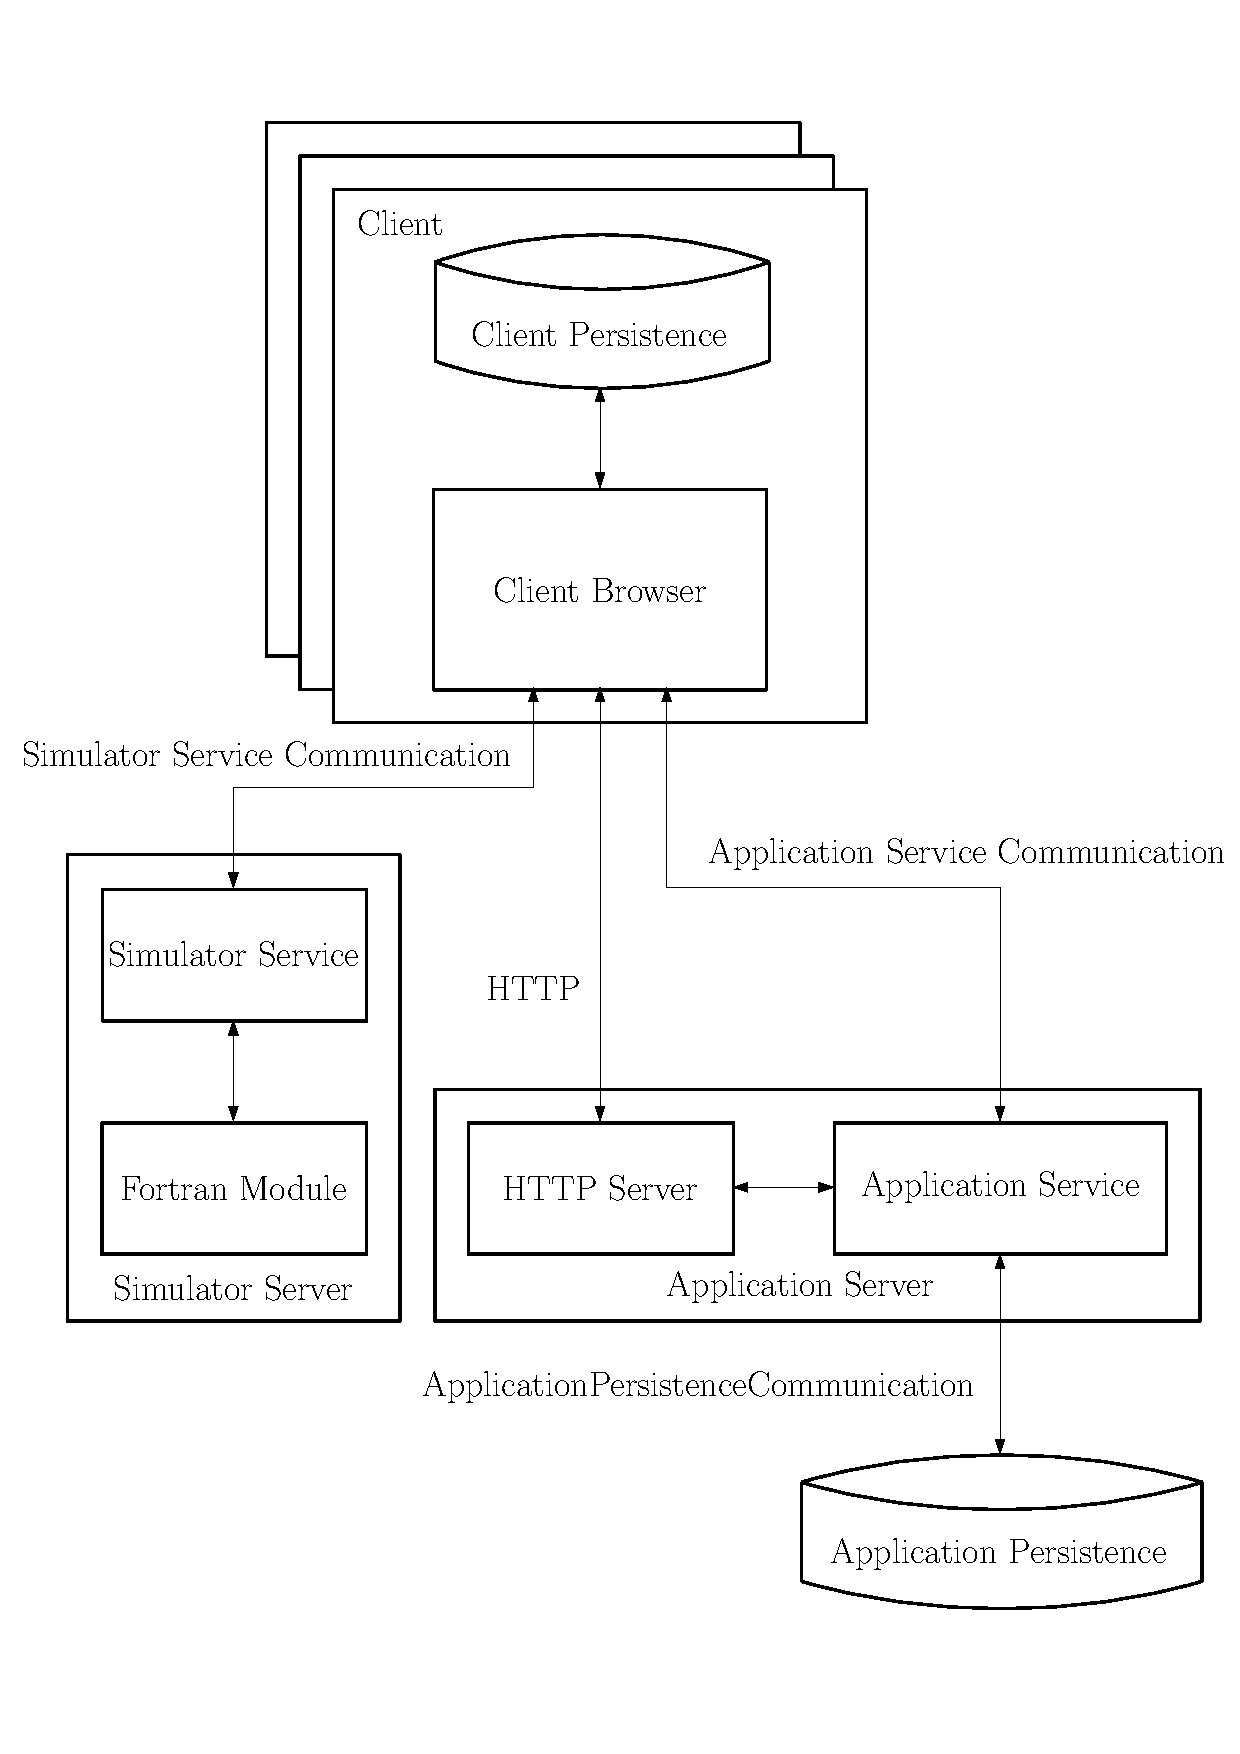
\includegraphics[scale=0.5]{SoftwareTiers}
\caption{The different tiers of the system}
\end{figure}


\chapter{Specific requirements}
\label{chap:specreq}
This chapter lists all specific software requirements of the application to be developed, both functional and non-functional requirements. The requirements are categorised according to the interface they belong to, as described in section \ref{sec:moddesc}.

Each requirement has a specific priority, based on the MoSCoW model \cite{moscow}:

\begin{itemize}
    \item \emph{must have}; requirements with this priority are essential for the product, and must be implemented.
    \item \emph{should have}; requirements with this priority are not essential for the product to work. However, they are nearly as important as the \emph{must have}'s and are therefore expected to be implemented.
    \item \emph{could have}; requirements with this priority are a nice addition to the product, and may be implemented, if time and budget allow this.
    \item \emph{won't have}; requirements with this priority will not be implemented in this version of the product, but may be nice to implement in future versions.
\end{itemize}

\noindent Only those user requirements from the URD \cite{urd} with a priority higher than \emph{won't have} will be translated to software requirements in this chapter.

\fpstartparagraph{} In some of the requirements in this section, the term ``fast enough" is mentioned: for a precise definition, refer to chapter 6 of the ADD \cite{add}.

% Functional requirements --------------------------------------------------------------------------------------------------------
\section{Functional requirements}
\label{sec:funcreq}
This section lists the functional requirements for the \applicationname.

\subsection{HTTP Server}
\SRQ[HTTP-1]{must have}{The HTTP Server must be able to serve static files (files that are not dynamically generated) to the Client Browser.}

\subsection{Application Service}
\SRQ[AS-1]{must have}{The Application Service must be able to retrieve all the available mixers from the Application Persistence.}
\SRQ[AS-2]{must have}{The Application Service must be able to send all available mixers to the Client Browser.}
\SRQ[AS-3]{must have}{The Application Service must allow for adding new mixers to the Application Persistence.} %CNR13
\SRQ[AS-5]{must have}{The Application Service must allow for removing existing mixers from the Application Persistence.}
\SRQ[AS-6]{must have}{The Application Service must be able to provide all available geometries to the Client Browser.}
\SRQ[AS-7]{must have}{The Application Service must be able to act as a relay between the Client Browser and the Simulation Service.}

\subsection{Application Persistence Communication}
\SRQ[APC-1]{must have}{The Application Persistence Communication must be able to access all the data from the Application Persistence.}
\SRQ[APC-2]{must have}{The Application Persistence Communication must be fast enough to serve the data from the Application Persistence to the Application Service.}

\subsection{Application Persistence}
\SRQ[AP-1]{must have}{The Application Persistence must deliver all saved mixers to the Application Service.}
\SRQ[AP-2]{must have}{The Application Persistence must be able to save new mixers provided by the Application Service.}
\SRQ[AP-5]{must have}{The System Administrator is able to add new mixer types for a geometry.}
\SRQ[AP-6]{must have}{The System Administrator is able to remove mixer types for a geometry.}

\subsection{Application Service Communication}
\SRQ[ASC-1]{must have}{The Application Service Communication must be able to access all the functionality from the Application Service.}
\SRQ[ASC-2]{must have}{The Application Service Communication must be fast enough to provide the functionality from the Application Service to the Client Browser.}

\subsection{Client Browser}
\subsubsection{Change the drawing tool}
The user can change the drawing tool that is used to paint on the canvas. The current shape (circle and square) and size of the drawing tool is displayed on the user interface. The user interface contains options to change the current shape and size of the drawing tool.

\SRQ[shapedraw]{must have}{The user interface displays the shape of the tool that is currently selected.} % CPR7
\SRQ[CB-12]{should have}{The user interface displays the size of the tool that is currently selected.} % CPR10
\SRQ[circleshaped]{must have}{A circle-shaped drawing tool can be selected on the graphical user interface.} % CPR7
\SRQ[squareshaped]{should have}{A square-shaped drawing tool can be selected on the graphical user interface.} % CPR9
\SRQ[CB-13]{should have}{A graphical user interface is present to adjust the size of the current tool.} % CPR10

\subsubsection{Defining an initial concentration distribution}
The user can select a circle or square-shaped drawing tool to draw with. He can draw on the canvas by swiping with his finger or drawing with the mouse. In addition, the user can reset the drawn distribution to a completely white concentration distribution.

\SRQ[CB-2]{must have}{A graphical interface is present to select the colour (black or white) to paint with for the initial concentration distribution.} % CPR6
\SRQ[CB-3]{must have}{A graphical interface is present to define an initial concentration distribution with the selected color on the canvas. It must be possible to define this distribution by means of ``painting'' on the canvas.} % CPR6
\SRQ[CB-4]{must have}{If the circle-shaped drawing tool in \srqref{circleshaped} is selected, this tool will be used when the canvas is ``painted''.} % CPR7, los omdat de square een lagere prioriteit heeft in het URD
\SRQ[CB-6]{should have}{If the square-shaped drawing tool in \srqref{squareshaped} is selected, this tool will be used when the canvas is ``painted''.}% CPR9
\SRQ[CB-5]{must have}{A graphical user interface is present to reset the current initial concentration distribution to a completely white state.} % CPR8

\subsubsection{Select a geometry, mixer and initial concentration distribution}
The user can select a rectangular mixer geometry. Then the user can select a mixer that can operate on the selected geometry and a initial concentration distribution. There are three types of initial concentration distributions that the user can choose from. The first type is a \texttt{blank} concentration distribution, which simply means that the user will be presented with a clean canvas when this option is selected. The second type is a \texttt{load} option, so the user can load previously saved concentration distributions that are stored on their device. The third type of
concentration distribution is a \texttt{predefined} distribution, meaning that the user can choose from a few predefined distributions that are already present in the application. The selected concentration distribution is then loaded onto the canvas. This translates to the following software requirements:

\SRQ[CB-7]{must have}{The application contains a graphical interface to select an initial mixer, geometry and options for the initial concentration distribution.} % CPR1
\SRQ[selgeomrec]{must have}{A \texttt{rectangle} geometry can be selected in the user interface.} % CPR1
\SRQ[selmixer]{must have}{If a geometry is selected, a user interface is presented to select an appropriate mixer.} % CPR2
\SRQ[selgeomsq]{should have}{A \texttt{square} geometry can be selected in the user interface.}  % CPR3
\SRQ[selgeomcir]{could have}{A \texttt{circle} geometry can be selected in the user interface.}  % CPR4
\SRQ[selgeomjb]{could have}{A \texttt{journal bearing} geometry can be selected in the user interface.}  % CPR5
\SRQ[CB-8]{must have}{After a geometry and appropriate mixer is slected in the user interface, a blank canvas can be selected and loaded.} % CPR6
\SRQ[prevsaved]{should have}{After a geometry and appropriate mixer is slected in the user interface, a list of all previously saved concentration distribution can be retrieved in the user interface.} % CPR13
\SRQ[CB-9]{should have}{After the list of concentration distribution from \srqref{prevsaved} is presented, a previously saved concentration distribution can be selected and loaded onto the canvas.} % CPR13
\SRQ[predef]{could have}{After a geometry and appropriate mixer is slected in the user interface, a list of all predefined concentration distribution can be retrieved in the user interface.} % CPR14
\SRQ[CB-10]{could have}{After the list of concentration distribution from \srqref{predef} is presented, a predefined concentration distribution can be selected and loaded onto the canvas.} % CPR14

\subsubsection{Define mixing protocol for specific geometries}
A mixing protocol consists of movements of the geometry (if applicable), and how long these movements are executed. Different movement types are possible for each geometry. A step of a mixing protocol has a certain duration (the step size, $D$). This duration $D$ can be any multiple of $0.25$. If a value is not a multiple of $0.25$, it will be rounded to the nearest valid value. For example, $4.2$ is rounded up to $4.25$, while $4.1$ is rounded down to $4$. Each movement is performed for $D$ time units, which can be set using \srqref{stepsize}. Depending on the geometry, a step has additional parameters signifying which part moves and how:

\fpstartparagraph{} For the \emph{rectangular} or \emph{square} geometries, a wall movement is defined by either $T$ or $B$, denoting a movement of the top or bottom wall, respectively. These movements can be combined with a $L$ or $R$ denoting whether the wall is moving left or right. This means there are four movement modifiers: $TL$, $TR$, $BL$ and $BR$.

The \emph{circular} geometry only supports one (unnamed) modifier.

For the \emph{journal bearing} geometry, movements are defined by rotating the outer or inner circle. The outer circle is denoted with an $O$ and the inner circle is denoted with an $I$. These modifiers can be combined with modifiers denoting the direction of the rotation, $R$ and $L$. This results in four possible modifiers: $OL$, $OR$, $IL$ and $IR$.

The user interface will contain options to input modifiers where appropriate and to indicate the step-size associated with those modifiers.

\fpstartparagraph{} A graphical interface is present to define how many times the current protocol should be run when the simulation has started.

\SRQ[stepsize]{must have}{ % CPR20
    A graphical user interface is present to associate a valid step-size (as defined above) to a step.
}

\SRQ[protocolrepeat]{must have}{ % CPR21
    A graphical user interface is present to indicate how many times the currently defined protocol should be executed when the simulation starts.
}

\SRQ[CB-14]{must have}{ % CPR17a, CPR25a, CPR26a, CPR27a
    A graphical user interface is present to associate a valid step-modifier (as defined above) to a step.
}

\SRQ[CB-15]{must have}{ % CPR17b, CPR25b, CPR26b, CPR27b
    A graphical user interface is present to add and remove steps to the protocol.
}

\SRQ[startMixing]{must have}{ % CPR29a
    If a geometry, a mixer, an initial distribution and a protocol are present, a graphical user interface must be available to execute the actual mixing simulation.
}

\SRQ[CB-16]{must have}{ % CPR19
    A grahpical user interface is present to reset the currently defined protocol, thereby removing all currently defined steps.
}

\subsubsection{Execute mixing runs}
The user can choose to execute a single step of a mixing protocol, by defining a single step. This is done by choosing one wall movement and its duration. This invokes \srqref{startMixing}, \srqref{sendParams}, \srqref{execMixing}, \srqref{returnParams} and \srqref{visResults}.

\SRQ[CB-17]{must have}{ % CPR18
    After selecting a geometry, a mixer, an initial distribution and a single step, the user can execute a mixing run with this single step.}

\subsubsection{Visualising the results}
The concentration distribution resulting from a mixing simulation is visualised in the user interface, using the canvas that was originally used to draw the initial concentration distribution. The performance results are visualised in a graph.

\SRQ[visResults]{must have}{ % CPR29e
    Concentration distributions can be drawn on the client's canvas.
}

\SRQ[CB-16-2]{must have}{ % CPR29f
    Performance results can be plotted in a graph.
}

\subsection{ClientPersistence}
\SRQ[CP-0]{should have}{The client persistence is capable of storing concentration distributions, mixing protocols and associated mixers and geometries. Results of a mixing run can also be stored.} % CPR11

\subsubsection{Managing mixing protocols}
To manage mixing protocols, the user can save and load the mixing protocols they have created. It is also possible to load a predefined mixing protocol.

\SRQ[CP-1]{should have}{A graphical user interface is present to save the concentration distribution currently drawn on the canvas to the ClientPersistence.} % CPR11

\SRQ[CP-2]{should have}{ % CPR22
    A graphical user interface is present to save the currently defined mixing protocol to the ClientPersistence.
}

\SRQ[CP-3]{should have}{ % CPR23
    A graphical user interface is present to view all saved mixing protocols and remove a mixing protocol.
}

\SRQ[CP-4]{should have}{ % CPR24
    A graphical user interface is present to view all saved mixing protocols appropriate to the currenctly selected geometry. A mixing protocol can be selected from this list and loaded into the current mixing protocol.
}

\SRQ[CP-5]{could have}{ % CPR28
    After \srqref{selgeomrec}, \srqref{selgeomsq}, \srqref{selgeomcir} or \srqref{selgeomjb}, the user can load a predefined mixing protocol. This opens a menu containing all suitable predefined mixing protocols for the selected geometry. Pressing the name of one such protocol selects it, which means it will be loaded into the application. After this it can be changed or used for simulation immediately.
}

\subsubsection{Save and remove mixing runs}
\SRQ[CP-6]{must have}{ % CPR30
    After the mixing has been executed, a graphical user interface is present to save the mixing run. That is, the resulting concentration distribution of the run is saved, the mixing protocol is saved, the performance result of the mixing simulation is saved and the used geometry and mixer are saved.
}

\SRQ[CP-7]{must have}{ % CPR31
    A list with previously saved mixing runs can be viewed on the user interface, and a saved mixing run can be selected and removed.
}

\subsubsection{Save an initial concentration distribution}
\SRQ[savedistr]{should have}{A graphical user interface is present to save the concentration distribution currently displayed on the canvas.} % CPR11
\SRQ[savename]{should have}{During the \srqref{savedistr} action a name for the concentration distribution can be inputted.} % CPR11
\SRQ[savebutton]{should have}{After specifying a name in \srqref{savename}, the concentration distribution can be saved to the ClientPersistence under the inputted name.} % CPR11
\SRQ[CP-9]{should have}{If the specified name from \srqref{savename} is already taken, a graphical user interface is present to overwrite the previously saved concentration distribution.} % CPR11
\SRQ[CP-10]{should have}{The saving process can be cancelled at any time.} % CPR11

\subsubsection{Load previously saved concentration distribution}
\SRQ[loaddistbutton]{should have}{A graphical user interface is present to initiate the loading of a previously saved concentration distribution.} % CPR13
\SRQ[loadlist]{should have}{After the loading process from \srqref{loaddistbutton} has been initiated, a list of previously saved concentration distributions is presented.} % CPR13
\SRQ[loadload]{should have}{In the list from \srqref{loadlist}, a previously saved distribution can be selected.}
\SRQ[CP-14]{should have}{A concentration distribution (for example the one selected in \srqref{loadload}) can be loaded into the canvas.}

\subsubsection{Remove previously saved concentration distributions}
\SRQ[removeinit]{should have}{A user interface is present to initiate the removal of a previously saved concentration distribution.} % CPR12
\SRQ[listsaved]{should have}{After the removal action from \srqref{removeinit} has begun, the user interface will present a list of previously saved concentration distributions.} % CPR12
\SRQ[selectremove]{should have}{After the list from \srqref{listsaved} is shown on the user interface, one or more previously saved concentration distributions can be selected for removal.} % CPR12
\SRQ[suremessage]{should have}{If an item from \srqref{selectremove} is selected for removal, a confirmation will be shown before the removal commences.} % CPR12
\SRQ[nosaveddistr]{should have}{If no distributions have been saved yet, and \srqref{removeinit} has been initiated, a message will be shown to inform the user that no items can currently be removed.} % CPR12+13
\SRQ[insuffrights]{should have}{If no access rights have been provided to the application, a \emph{Insufficient access rights} error message is shown when \srqref{removeinit} is initiated.} % CPR12

\subsubsection{Exporting results}
It is possible to save an image of the results of a performed mixing run to the disk of the Client. This can be a image of the resulting concentration distribution, an animation of several intermediate concentration distributions (as indicated by the step-repeat from \srqref{protocolrepeat}) or a graph displaying the performance of a mixing run (a performance point is generated for each time the protocol was repeated using \srqref{protocolrepeat}).

\SRQ[distimg]{should have}{A graphical user interface is present to export an image of the current concentration distribution.}
%CPR33
\SRQ[gengraph]{should have}{A graphical user interface is present to export an image of the current performance graph.}
%CPR35&37
\SRQ[gendist]{could have}{A graphical user interface is present to export an animation or still frame of the current mixing protocol.}

%CPR39
\SRQ[exportname]{should have}{The generated image or animation from \srqref{gengraph} and \srqref{gendist} is presented to the ClientBrowser and the ClientBrowser is expected to handle further steps in order to save the image or animation to the disk.}
%CPR33&35&37&39

\subsubsection{Loading results}
Previously saved results can be loaded into the application.

\SRQ[initload]{should have}{A graphical user interface should be present to initiate the loading of previously saved results. The interface shows a list of these saved results.}
%CPR30&36
\SRQ[selectload]{should have}{After the loading action from \srqref{initload} has been initiated, a saved result can be selected to load.}
%CPR30&36
\SRQ[displayload]{should have}{When \srqref{selectload} is executed, the concentration distribution resulting from the saved mixing simulation is loaded and the performance graph is displayed.}
%CPR30&36
\SRQ[CP-28]{should have}{A graphical user interface should be present to load multiple results to create a performance graph where multiple results are overlayed. The result of this graph can be saved to the disk.}
%CPR30&36

\subsubsection{Language selection}
It is possible to change the language of the application. The standard language is English from \srqref{englan}, and it should be relatively easy to add other languages.
\SRQ[selLang]{could have}{
  A graphical user interface is present to select one of the available languages for the application (these languages are \srqref{englan} and \srqref{dutlan}).
}

\subsubsection{Requirements regarding the presentation of results}
The user is able to get the distribution that resulted from executing his mixing run. In addition, the mixing performance is given after each mixing step. He is also able to save and export these results. The user interface must be able to support this functionality.

\SRQ[SSC-3]{must have}{A graphical user interface is present to show the mixing protocol of a loaded mixing run.}
%CPR32
\SRQ[SSC-4]{must have}{A graphical user interface is present to view the performance graph of a loaded mixing run.}
%CPR34
\SRQ[SSC-6]{could have}{A graphical user interface is present to view an animation of a loaded mixing run, if the user selected the animate option.}
%CPR38

\subsection{Simulator Service Communication}

\SRQ[sendParams]{must have}{ % CPR29b
    The parameters (initial concentration distribution, geometry, mixing protocol, mixer and number of protocol applications) can be sent from the Application Service to the Simulation Service through the Simulator Service Communication channel.
}

\SRQ[returnParams]{must have}{ % CPR29d
    The results of a mixing simulation can be sent from the Simulator Service to the Application Service through the Simulator Service Communication.
}

\subsection{Simulator Service}
\SRQ[execMixing]{must have}{ %CRP29c2
     The server executes the mixing run using the parameters received from the Simulator Service Communication. These parameters are passed as input to the Fortran implementation.
}
\SRQ[returnMixing]{must have}{
	The server can return the results from a mixing simulation it received from the fortran module to the Application Service through the Simulator Service Communication.
}

\subsubsection{Information exchange}
The Simulator Service must be able to send and receive matrix files from the Client Browser and to the Fortran Module. These matrices specify the characteristics of the mixers.

\SRQ[SS-2]{must have}{The Simulator Service must be able to receive protocol information from the Client Browser through the Application Service.}
\SRQ[SS-4]{must have}{The Simulator Service must be able to pass protocol information to the Fortran Module.}

\subsection{Fortran Module}
\SRQ[FM-1]{must have}{The Fortran Module must accept input (matrix name, protocol information) from the Simulator Service.}
\SRQ[FM-2]{must have}{The Fortran Module must provide output (vectors) to the Simulator Service.}
\SRQ[FM-3]{must have}{The Fortran Module must have knowledge of all the geometries and mixers used in the application. This knowledge is not automatically transferred from the application to the Fortran module.}

% Non-functional requirements ----------------------------------------------------------------------------------------------------
\section{Non-functional requirements}
\label{sec:nonfuncreq}

\subsection{Performance}
\SRQ[NONF-1]{must have}{Waiting time between submitting input and receiving output is around 5 seconds on average.}
%CNR10

\SRQ[NONF-2]{should have}{Waiting time between submitting input and receiving output is around 3 seconds on average.}
%CNR11

\SRQ[NONF-3]{could have}{Waiting time between submitting input and receiving output is around 1 second on average.}
%CNR12

\subsection{Interface}
\SRQ[englan]{must have}{An English interface is available.}
%CPR40

\SRQ[dutlan]{should have}{A Dutch interface is available.}
%CPR41

\subsection{Portability}
\SRQ[NONF-6]{must have}{The application runs on iOS Safari version 6.0 and higher.}
%CNR1

\SRQ[NONF-7]{should have}{The application runs on Firefox version 20 and higher.}
%CNR2

\SRQ[NONF-8]{should have}{The application runs on Google Chrome version 26 and
higher.}
%CNR3

\SRQ[NONF-9]{could have}{The application runs on Internet Explorer version 10 and higher.}
%CNR4

\SRQ[NONF-10]{could have}{The application runs on Safari version 6.0 and higher.}
%CNR5

\SRQ[NONF-11]{must have}{The application runs on devices running on iOS version 6 and higher.}
%CNR7

\SRQ[NONF-12]{should have}{The application runs on devices running on Android version 4.0 and higher.}
%CNR8

\SRQ[NONF-13]{could have}{The application runs on devices running on Windows 8.}
%CNR9


\chapter{Reference}
This chapter describes various parts of the \applicationname{}. For each reference, a short functional description is provided, along with warnings and errors. Furthermore, examples and related references are listed for each item.

\section{Cell Browser}
  \subsection*{Functional description}
  \todo{What the operation(command, menu item, button, ...) achieves}

  \subsection*{Cautions and warnings}
  \todo{A list of cautions and warnings that apply to the operation}

  \subsection*{Formal description}
  \todo{A formal description of what the operation does and how it is used: required parameters, optional parameters, defaults, syntax and semantics}

  \subsection*{Examples}
  \todo{One or more examples of the use of the operation.}

  \subsection*{Possible errors}
  \todo{A list of all possible errors for this operation and their causes}

  \subsection*{Related operations}
  \todo{References to, for example, operations to complete a task or logically related operations.}

\section{Drawing Area}
  \subsection*{Functional description}
  \todo{What the operation(command, menu item, button, ...) achieves}

  \subsection*{Cautions and warnings}
  \todo{A list of cautions and warnings that apply to the operation}

  \subsection*{Formal description}
  \todo{A formal description of what the operation does and how it is used: required parameters, optional parameters, defaults, syntax and semantics}

  \subsection*{Examples}
  \todo{One or more examples of the use of the operation.}

  \subsection*{Possible errors}
  \todo{A list of all possible errors for this operation and their causes}

  \subsection*{Related operations}
  \todo{References to, for example, operations to complete a task or logically related operations.}

\section{Main Menu}
  \subsection*{Functional description}
  \todo{What the operation(command, menu item, button, ...) achieves}

  \subsection*{Cautions and warnings}
  \todo{A list of cautions and warnings that apply to the operation}

  \subsection*{Formal description}
  \todo{A formal description of what the operation does and how it is used: required parameters, optional parameters, defaults, syntax and semantics}

  \subsection*{Examples}
  \todo{One or more examples of the use of the operation.}

  \subsection*{Possible errors}
  \todo{A list of all possible errors for this operation and their causes}

  \subsection*{Related operations}
  \todo{References to, for example, operations to complete a task or logically related operations.}

\section{Select Tool Menu}
  \subsection*{Functional description}
  \todo{What the operation(command, menu item, button, ...) achieves}

  \subsection*{Cautions and warnings}
  \todo{A list of cautions and warnings that apply to the operation}

  \subsection*{Formal description}
  \todo{A formal description of what the operation does and how it is used: required parameters, optional parameters, defaults, syntax and semantics}

  \subsection*{Examples}
  \todo{One or more examples of the use of the operation.}

  \subsection*{Possible errors}
  \todo{A list of all possible errors for this operation and their causes}

  \subsection*{Related operations}
  \todo{References to, for example, operations to complete a task or logically related operations.}

\section{Distributions Menu}
  \subsection*{Functional description}
  \todo{What the operation(command, menu item, button, ...) achieves}

  \subsection*{Cautions and warnings}
  \todo{A list of cautions and warnings that apply to the operation}

  \subsection*{Formal description}
  \todo{A formal description of what the operation does and how it is used: required parameters, optional parameters, defaults, syntax and semantics}

  \subsection*{Examples}
  \todo{One or more examples of the use of the operation.}

  \subsection*{Possible errors}
  \todo{A list of all possible errors for this operation and their causes}

  \subsection*{Related operations}
  \todo{References to, for example, operations to complete a task or logically related operations.}
  
\section{Results Menu}
  \subsection*{Functional description}
  \todo{What the operation(command, menu item, button, ...) achieves}

  \subsection*{Cautions and warnings}
  \todo{A list of cautions and warnings that apply to the operation}

  \subsection*{Formal description}
  \todo{A formal description of what the operation does and how it is used: required parameters, optional parameters, defaults, syntax and semantics}

  \subsection*{Examples}
  \todo{One or more examples of the use of the operation.}

  \subsection*{Possible errors}
  \todo{A list of all possible errors for this operation and their causes}

  \subsection*{Related operations}
  \todo{References to, for example, operations to complete a task or logically related operations.}

\section{Define Protocol Menu}
  \subsection*{Functional description}
  \todo{What the operation(command, menu item, button, ...) achieves}

  \subsection*{Cautions and warnings}
  \todo{A list of cautions and warnings that apply to the operation}

  \subsection*{Formal description}
  \todo{A formal description of what the operation does and how it is used: required parameters, optional parameters, defaults, syntax and semantics}

  \subsection*{Examples}
  \todo{One or more examples of the use of the operation.}

  \subsection*{Possible errors}
  \todo{A list of all possible errors for this operation and their causes}

  \subsection*{Related operations}
  \todo{References to, for example, operations to complete a task or logically related operations.}

\section{Protocols Menu}
  \subsection*{Functional description}
  \todo{What the operation(command, menu item, button, ...) achieves}

  \subsection*{Cautions and warnings}
  \todo{A list of cautions and warnings that apply to the operation}

  \subsection*{Formal description}
  \todo{A formal description of what the operation does and how it is used: required parameters, optional parameters, defaults, syntax and semantics}

  \subsection*{Examples}
  \todo{One or more examples of the use of the operation.}

  \subsection*{Possible errors}
  \todo{A list of all possible errors for this operation and their causes}

  \subsection*{Related operations}
  \todo{References to, for example, operations to complete a task or logically related operations.}

%-------------------------------------------------------------------------------------------------
\section{Save Item Panel}
\label{sec:saveitem}
  \subsection*{Functional description}
  %What the operation(command, menu item, button, ...) achieves
  This panel contains a text box. Furthermore it provides functionality to save an item, and to cancel the operation.

  \subsection*{Cautions and warnings}
  %A list of cautions and warnings that apply to the operation
  \begin{itemize}
  \item Saving the file is only possible with a new of at least 1 character.
  \item File names can be no longer than 30 characters.
  \item Characters other then the letters of the Latin script, the numbers 0 through 9 and spaces cannot be used in file names.
  \item File names cannot start with a space.
  \end{itemize}

  \subsection*{Formal description}
  %A formal description of what the operation does and how it is used: required parameters, optional parameters, defaults, syntax and semantics
    \begin{tabularx}{\textwidth}{XXX}
    \toprule
    \emph{Operation} & \emph{Steps} & \emph{Results} \\
    \midrule
    Insert (part of) a file name & Press inside the text box. Insert any of the valid characters (see section \textbf{Cautions and warnings}). & The chosen character appears in the text box. \\
    \midrule
    Remove (part of) a file name & Press inside the text box. Press \emph{backspace}. & The last character of the name disappears. \\
    \midrule
    Save an item & Press the \emph{Save} button. & The panel closes, and a \emph{Save successful} message appears and disappears again. \\
    \midrule
    Cancel operation & Press the \emph{Cancel} button. & The panel is closed. \\
    \bottomrule
\end{tabularx}

  \subsection*{Possible errors}
  %A list of all possible errors for this operation and their causes
  \begin{description}
  \item[The message \emph{This name is already in use} is shown.] Another file has already been saved with this name. Also see section \ref{sec:overwriteitem}.
  \end{description}

  \subsection*{Related operations}
  %References to, for example, operations to complete a task or logically related operations.
   \begin{itemize}
   \item Section {sec:distmenu}
   \item Section {sec:resultsmenu}
   \item Section {sec:protmenu}
   \item Section {sec:overwriteitem}
  \end{itemize}

%-------------------------------------------------------------------------------------------------
\section{Overwrite Item Panel}
\label{sec:overwriteitem}
  \subsection*{Functional description}
  %What the operation(command, menu item, button, ...) achieves
  This panel shows the message \emph{This name is already in use. Choose whether to overwrite existing file or to cancel}. Furthermore it provides functionality to overwrite the file, or to cancel the operation.

  \subsection*{Cautions and warnings}
  %A list of cautions and warnings that apply to the operation
  \begin{itemize}
  \item After making use of the fuctionality to overwrite a file, it's not possible to retrieve the overwritten file.
  \end{itemize}

  \subsection*{Formal description}
  %A formal description of what the operation does and how it is used: required parameters, optional parameters, defaults, syntax and semantics
    \begin{tabularx}{\textwidth}{XXX}
    \toprule
    \emph{Operation} & \emph{Steps} & \emph{Results} \\
    \midrule
    Overwrite file & Press the \emph{Overwrite} button. & The panel is closed, and a \emph{Save successful} message appears and disappears again. \\
    \midrule
    Cancel operation & Press the \emph{Cancel} button. & The panel is closed, and the Save Item Panel (see section \ref{sec:saveitem}) is displayed again. \\
    \bottomrule
\end{tabularx}

  \subsection*{Possible errors}
  %A list of all possible errors for this operation and their causes
  \begin{description}
  \item[The message \emph{Local storage error} is shown.] Something went wrong with the the local storage of the browser.
  \item[The message \emph{Your storage is full. Please remove some items} is shown.] The browser can't store any more items. Remove items using the Remove Item Panel (see section \ref{sec:removeitem}).
  \item[The message \emph{An unknown error has occurred} is shown.] Cause unknown.
  \end{description}

  \subsection*{Related operations}
  %References to, for example, operations to complete a task or logically related operations.
   \begin{itemize}
   \item Section {sec:distmenu}
   \item Section {sec:resultsmenu}
   \item Section {sec:protmenu}
   \item Section {sec:saveitem}
  \end{itemize}

%-------------------------------------------------------------------------------------------------
\section{Load Item Panel}
\label{sec:loaditempanel}
  \subsection*{Functional description}
  %What the operation(command, menu item, button, ...) achieves
  This panel provides functionality for loading items. It provides functionality to load the shown items, and to close the panel.

  \subsection*{Cautions and warnings}
  %A list of cautions and warnings that apply to the operation
  \begin{itemize}
  \item This panel shows the text \emph{No saved files} when no items have been saved yet.
  \end{itemize}

  \subsection*{Formal description}
  %A formal description of what the operation does and how it is used: required parameters, optional parameters, defaults, syntax and semantics
    \begin{tabularx}{\textwidth}{XXX}
    \toprule
    \emph{Operation} & \emph{Steps} & \emph{Results} \\
    \midrule
    Load an item & Press the one of the items in the list & The selected item is loaded in the drawing area (distribution), define protocol menu (protocol) or both (mixing result). \\
    \midrule
    Close panel & Press the \emph{Close} button. & The panel is closed. \\
    \bottomrule
\end{tabularx}

  \subsection*{Possible errors}
  %A list of all possible errors for this operation and their causes
  None.

  \subsection*{Related operations}
  %References to, for example, operations to complete a task or logically related operations.
   \begin{itemize}
   \item Section {sec:distmenu}
   \item Section {sec:resultsmenu}
   \item Section {sec:protmenu}
  \end{itemize}

%-------------------------------------------------------------------------------------------------
\section{Remove Item Panel}
\label{sec:removeitem}
  \subsection*{Functional description}
  %What the operation(command, menu item, button, ...) achieves
  This panel provides functionality for removing items. It provides functionality to remove the shown items, and to close the panel.

  \subsection*{Cautions and warnings}
  %A list of cautions and warnings that apply to the operation
  \begin{itemize}
  \item This panel shows the text \emph{No saved files} when no items have been saved yet.
  \end{itemize}

  \subsection*{Formal description}
  %A formal description of what the operation does and how it is used: required parameters, optional parameters, defaults, syntax and semantics
    \begin{tabularx}{\textwidth}{XXX}
    \toprule
    \emph{Operation} & \emph{Steps} & \emph{Results} \\
    \midrule
    Remove an item & Press the \texttt{X} next to one of the items. &  The chosen item disappears from the list, and a \emph{Delete successful} message appears and disappears again. \\
    \midrule
    Close panel & Press the \emph{Close} button. & The panel is closed. \\
    \bottomrule
\end{tabularx}

  \subsection*{Possible errors}
  %A list of all possible errors for this operation and their causes
  None.

  \subsection*{Related operations}
  %References to, for example, operations to complete a task or logically related operations.
   \begin{itemize}
   \item Section {sec:distmenu}
   \item Section {sec:resultsmenu}
   \item Section {sec:protmenu}
  \end{itemize}
  
%-------------------------------------------------------------------------------------------------
\section{Compare Performance Panel}
\label{sec:compareperf}
  \subsection*{Functional description}
  %What the operation(command, menu item, button, ...) achieves
  This panel shows a list of all saved mixing runs. Furthermore it contains options to select one or more of these mixing runs, to compare the  performance of the selected runs and to cancel the operation.

  \subsection*{Cautions and warnings}
  %A list of cautions and warnings that apply to the operation
  \begin{itemize}
  \item This panel shows the text \emph{No saved files} and doesn't have the option to compare when no mixing runs have been saved yet. Also see section \ref{sec:resultsmenu}.
  \end{itemize}

  \subsection*{Formal description}
  %A formal description of what the operation does and how it is used: required parameters, optional parameters, defaults, syntax and semantics
    \begin{tabularx}{\textwidth}{XXX}
    \toprule
    \emph{Operation} & \emph{Steps} & \emph{Results} \\
    \midrule
    Select a result & Press a result that has a white or gray background. & The result is displayed in a white font and with a blue background. \\
    \midrule
    Deselect a result & Press a result that has a blue background. & The result is displayed in a black font and with a white or gray background. \\
    \midrule
    Compare performance of selected results & Press the \emph{Compare} button. & The \emph{Mixing Performance Graph Panel (Multiple)} is displayed. Also see section \ref{sec:mulperfgraph}. \\
    \midrule
    Cancel operation & Press the \emph{Cancel} button. & The panel is closed. \\
    \bottomrule
\end{tabularx}

  \subsection*{Possible errors}
  %A list of all possible errors for this operation and their causes
  None.

  \subsection*{Related operations}
  %References to, for example, operations to complete a task or logically related operations.
   \begin{itemize}
   \item Section {sec:resultsmenu}
   \item Section {sec:mulperfgraph}
  \end{itemize}

%-------------------------------------------------------------------------------------------------
\section{Mixing Performance Graph Panel (Single)}
\label{sec:singperfgraph}
  \subsection*{Functional description}
  %What the operation(command, menu item, button, ...) achieves
  This panel shows a figure with the performance graph of the last executed mixing run. Furthermore it contains options to export this figure and to close this panel.

  \subsection*{Cautions and warnings}
  %A list of cautions and warnings that apply to the operation
  \begin{itemize}
  \item The figure of the performance graphs doesn't display in Internet Explorer (all versions).
  \end{itemize}

  \subsection*{Formal description}
  %A formal description of what the operation does and how it is used: required parameters, optional parameters, defaults, syntax and semantics
    \begin{tabularx}{\textwidth}{XXX}
    \toprule
    \emph{Operation} & \emph{Steps} & \emph{Results} \\
    \midrule
    View performance of a single point & Press one of the points in the graph. & A popup appears with the performance value of this point. \\
    \midrule
    Export graph & Press the \emph{Export graph} button. & The default download window of your browser is displayed. \\
    \midrule
    Close panel & Press the \emph{Close} button. & The panel is closed. \\
    \bottomrule
\end{tabularx}

  \subsection*{Possible errors}
  %A list of all possible errors for this operation and their causes
  None.

  \subsection*{Related operations}
  %References to, for example, operations to complete a task or logically related operations.
   \begin{itemize}
   \item Section \ref{sec:defprot}
  \end{itemize}

%-------------------------------------------------------------------------------------------------
\section{Mixing Performance Graph Panel (Multiple)}
\label{sec:mulperfgraph}
  \subsection*{Functional description}
  %What the operation(command, menu item, button, ...) achieves
  This panel shows a figure with the performance graphs of one or more mixing runs. Furthermore it contains options to export this figure, to create a new figure with the performance of different mixing runs, and to close this panel.

  \subsection*{Cautions and warnings}
  %A list of cautions and warnings that apply to the operation
  \begin{itemize}
  \item The figure of the performance graphs doesn't display in Internet Explorer (all versions).
  \end{itemize}

  \subsection*{Formal description}
  %A formal description of what the operation does and how it is used: required parameters, optional parameters, defaults, syntax and semantics
    \begin{tabularx}{\textwidth}{XXX}
    \toprule
    \emph{Operation} & \emph{Steps} & \emph{Results} \\
    \midrule
    View performance of a single point & Press one of the points in the graph. & A popup appears with the performance value of this point. \\
    \midrule
    Export graph & Press the \emph{Export graph} button. & The default download window of your browser is displayed. \\
    \midrule
    Create new graph & Press the \emph{New comparison} button. & The panel from section \ref{sec:compareperf} is displayed. \\
    \midrule
    Close panel & Press the \emph{Close} button. & The panel is closed. \\
    \bottomrule
\end{tabularx}

  \subsection*{Possible errors}
  %A list of all possible errors for this operation and their causes
  \begin{description}
  \item[The panel shows a blank field with the text \emph{No data}] A comparison was made with no results selected. Also see section \ref{sec:compareperf}.\\
  \end{description}

  \subsection*{Related operations}
  %References to, for example, operations to complete a task or logically related operations.
   \begin{itemize}
   \item Section \ref{sec:resultsmenu}
   \item Section \ref{sec:compareperf}
  \end{itemize}

%-------------------------------------------------------------------------------------------------
\section{Toggle Menu Button}
\label{sec:togmenu}
  \subsection*{Functional description}
  %What the operation(command, menu item, button, ...) achieves
  This button is always shown in the top right corner of the application. It can be used to hide the menu bar when it is shown, and to show it again when it is hidden.

  \subsection*{Cautions and warnings}
  %A list of cautions and warnings that apply to the operation
  None.

  \subsection*{Formal description}
  %A formal description of what the operation does and how it is used: required parameters, optional parameters, defaults, syntax and semantics
  \begin{tabularx}{\textwidth}{XXX}
    \toprule
    \emph{Operation} & \emph{Steps} & \emph{Results} \\
    \midrule
    Hide menu & Press the blue circular button with a white \texttt{X} sign. & The menu bar on the right side of the application slides to the right until it isn't visible anymore. Simulatenously the blue circular button rotates until it shows a \texttt{+} sign.\\
    \midrule
    Show menu & Press the blue circular button with a white \texttt{+} sign. & The menu bar on the right side of the application appears and slides to the left until it's entirely visible. Simulatenously the blue circular button rotates until it shows an \texttt{X} sign. \\
    \bottomrule
\end{tabularx}

  \subsection*{Possible errors}
  %A list of all possible errors for this operation and their causes
  None.

  \subsection*{Related operations}
  %References to, for example, operations to complete a task or logically related operations.
  \begin{itemize}
  \item Section \ref{sec:drawingarea}
  \item Section \ref{sec:mainmenu}
  \item Section \ref{sec:selecttoolmenu}
  \item Section \ref{sec:distmenu}
  \item Section \ref{sec:resultsmenu}
  \item Section \ref{sec:defprot}
  \item Section \ref{sec:protmenu}
  \end{itemize}


% ============================================================
% Appendices
% ============================================================

\end{document}
